\begin{frame}[t]
    \frametitle{Applying Learning}
    Greedy search when $r \approx 0$, probabilistic when $r>0$:
    \[P(v_i|q,H) = \frac{e^{-d(v_i,q)/r}}{\sum_{v_j \in H}e^{-d(v_j,q)/r}}\]

    \onslide<2-3> {
    Applying $r=1$ and learning:
    \[P(v_i|q,H) = \frac{e^{<f(v_i), g(q)>}}{\sum_{v_j \in H}e^{<f(v_j),g(q)>}}\]\\
    }
    \onslide<3> {
    \noindent $f(v)$ is a function we wish to learn over $v \in S$, along with $g(q)$ over various queries.\\
    The functions are learned in tandem, as one will directly affect the results of the other.\\
    }
\end{frame}

\begin{frame}[t]
    \frametitle{Learning $f(v)$ and $g(q)$: Optimal Routing}
    Input: Given many examples $<v_1^*, q_1>, \dots <v_m^*, q_m>$\\
    Use BFS to find the $v_i$ which are closest to $v^*$.\\
    These vertices are likely to lead to $v^*$ for similar queries, so they are rated highly for $q$.
    \vspace{0.5em}

    \onslide<2-4> {
    Imitation Learning:\\
    Key Idea: We will make mistakes on new queries and need to recover. Imitate making those mistakes while learning.\\
    }
    \vspace{0.5em}

    \onslide<3-4> {
        Naive objective to maximize:
        \[E_{q,v^*} \sum_{v_i,H_i\in \text{Opt}(q)} \text{logP}(v_i|q,H_i,\theta)+ \text{logP}(v^*\in \text{TopK}|q,V,\theta)\]\\
    }
    \onslide<4> {
        Objective to maximize with imitation learning:
        \[E_{q,v^*} \sum_{v_i,H_i\in \text{Search}_\theta(q)} \text{logP}(v_i \in \text{Ref}(H_i)|q,H_i,\theta)+ \text{logP}(v^*\in \text{TopK}|q,V,\theta)\]
    }

\end{frame}

% \begin{frame}[t]
%     \frametitle{Problem to Solve}
%     \begin{center}
% 		\resizebox{\textwidth}{!}{
% 			%\begin{tikzpicture}
    \tikzstyle{node} = [circle, fill=lightgray!90!black, draw, thick]
    \tikzstyle{edge} = [thick]
    \tikzstyle{edit} = [fill=editcol]
    \tikzstyle{lift} = [fill=liftcol]

    \node (1) [node] {};
    \node (2) [node, above right=0.5cm and 0.3cm of 1] {};
    \node (3) [node, right=0.3cm of 2] {};
    \node (4) [node, above left=0.5cm and 0.3cm of 1] {};
    \node (5) [node, below=0.5cm of 2] {};

    \draw (1) edge [edge] (2);
    \draw (2) edge [edge] (3);
    \draw (2) edge [edge] (4);

    % First round of animation
    \onslide<1-2>{
        \draw (1) edge [edge] (4);
        \draw (2) edge [edge] (5);
    }

    \onslide<2-3>{
        \draw (3) edge [edge, dashed, color=addcol] (5) {};
    }

    \onslide<3>{
        \draw (1) edge [edge, color=removecol] (4);
        \draw (2) edge [edge, color=removecol] (5);
    }

    \onslide<4-5>{
        \draw (3) edge [edge] (5) {};
    }


\end{tikzpicture}
%             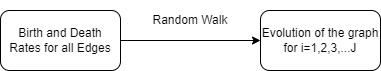
\includegraphics[]{figures/Inverse Problem Figure.jpg}
% 		}
% 	\end{center}

%     Forward Problem: Given a graph, $\hat{\alpha}$, and $\hat{\omega}$: compute states of the graph for $i=1,2, \dots J$
    
%     \vspace{1.0em}
%     Inverse Problem: Given a graph and $J$ states of the graph: compute $\hat{\alpha}$ and $\hat{\omega}$.
    
% \end{frame}

% \begin{frame}[t]

%     \frametitle{Defining the Inverse Problem}
    
%     \defproblem{Evolving Graph Model}
% 	{A graph $G$, $J$ states of the graph $F$, and a matrix $R$ containing the frequencies of each edge in $F$}
% 	{What mapping on the integers $q$ minimizes $\sum_{v_1,v_2 \in G}R[v_1][v_2](q(v_1) - q(v_2))^2$?}

%     \onslide<2-4> {
%         Problem: Since $q$ is not differentiable, this problem is intractable.\\
%         Solution: We relax $q$ to be a vector instead of a function
%     }

%     \onslide<3-4> {
%         \vspace{1.2em}
%         This leads to the form: $q^T\Delta_Rq$.\\
%         Note: $\Delta_R$ is the Laplacian matrix of $R$
%     }

%     \onslide<4> {
%         \vspace{1.2em}
%         Big problem: $q^T\Delta_Rq$ is a nonlinear (quadratic) inverse problem.
%     }

% \end{frame}

% \begin{frame}[t]
%     \frametitle{Solving the Quadratic Inverse Problem}

%     Problem to solve: $q^T\Delta_Rq$
    
%     \onslide<2-3>{
%         \vspace{1.2em}
%         One solution: eigenanalysis by cases on the matrix $\Delta_R$\\
%         Runtime: $O(n^3)$\\
%         By: Grindrod and Higham (2009)
%     }

%     \onslide<3>{
%         \vspace{1.2em}
%         My solution: convert to optimization, perform gradient descent\\
%         Derivative: $q^T(A + A^T)$\\
%         Compute the derivative and take a step towards it, then repeat.\\
%         Runtime: $O(sn^2)$, where $s$ is the number of steps to converge
%     }

% \end{frame}